% ------------------------------------------------------------------------
% file `main-bookexercise-5-exercise-body.tex'
%
%     exercise of type `bookexercise' with id `5'
%
% generated by the `exercise' environment of the
%   `xsim' package v0.21 (2022/02/12)
% from source `main' on 2026/10/17 on line 2316
% ------------------------------------------------------------------------
1. [判断]二叉查找树，也称二叉排序树、二叉搜索树。\\

2. [判断]平衡二叉树一定都是二叉查找树。\\

3. （某年408真题）下列二叉排序树中，满足平衡二叉树定义的是\underline{\hspace{1cm}}\\
\begin{center}
    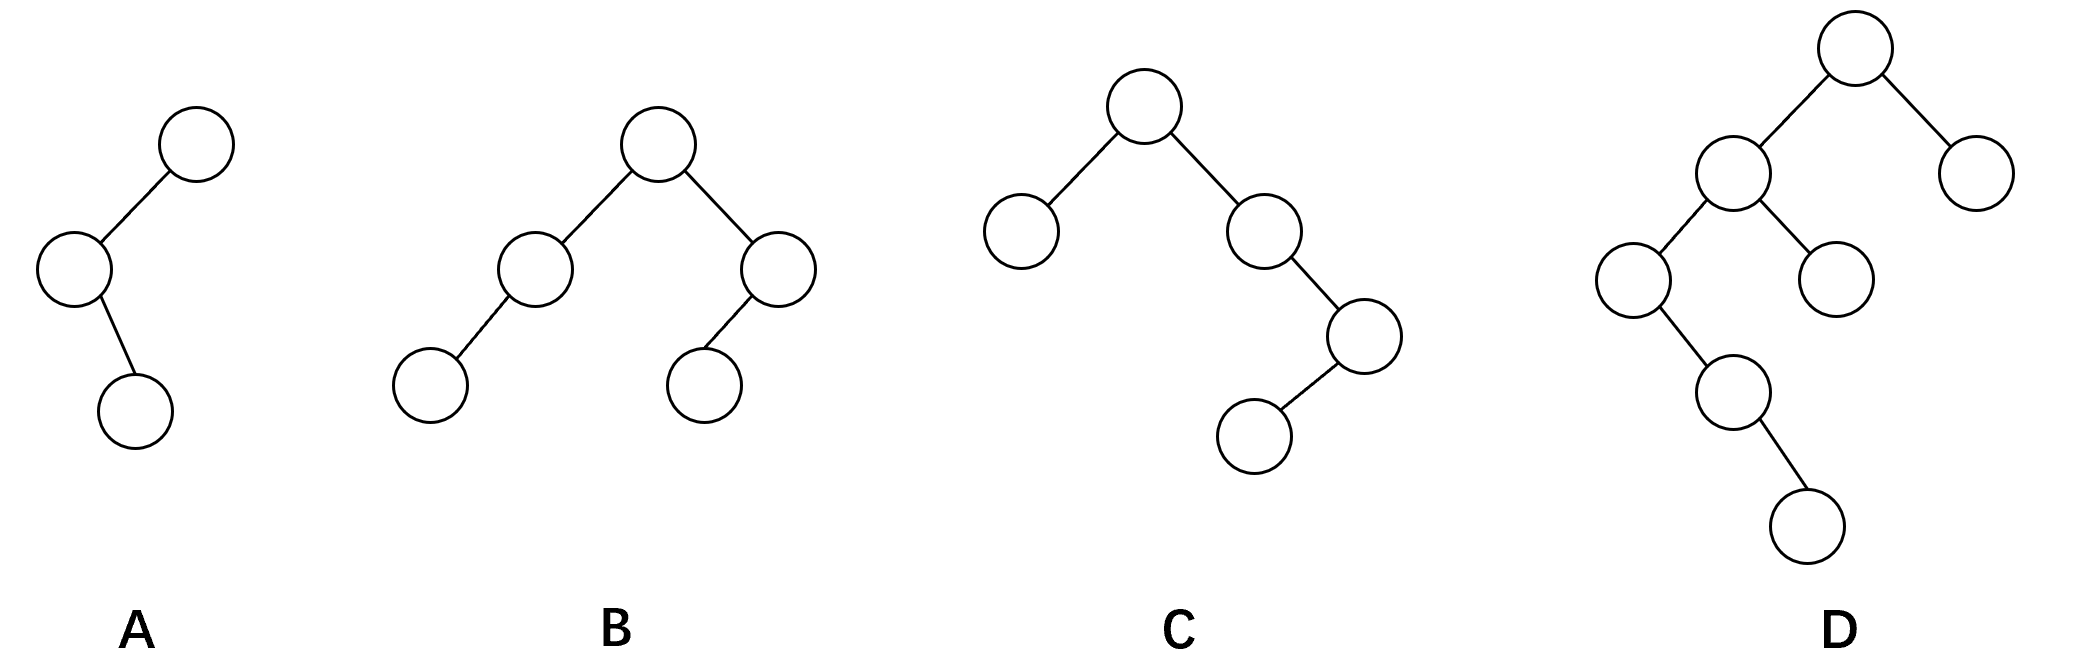
\includegraphics[width=0.81\textwidth]{assets/pics_and_ppts/ch4/09408_平衡二叉树定义.png}
\end{center}

\vspace{\baselineskip}

4. （某年408真题）对下列关键字序列，不可能构成二叉排序树中一条查找路径的是\underline{\hspace{1cm}}\\[0.5em]
\begin{tabular}{ll}
    A. 95, 22, 91, 24, 94, 71 & B. 92, 20, 91, 34, 88, 35\\
    C. 21, 89, 77, 29, 36, 38 & D. 12, 25, 71, 68, 33, 34\\
\end{tabular}

\vspace{\baselineskip}

5. （某年408真题）在下图所示的平衡二叉树中插入关键字48后得到一棵新的平衡二叉树，在新平衡二叉树中，关键字37所在节点的左、右子节点中保存的关键字分别是\underline{\hspace{1cm}}\\[0.5em]
\begin{center}
    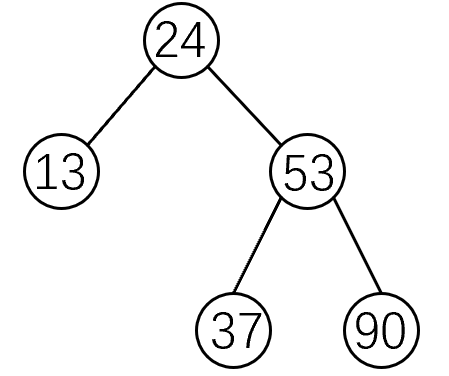
\includegraphics[width=0.21\textwidth]{assets/pics_and_ppts/ch4/10408_平衡二叉树插入后37的左右孩子值.png}
\end{center}

\begin{tabular}{llll}
    A. 13, 48 & B. 24, 48 & C. 24, 53 & D. 24, 90
\end{tabular}

\vspace{\baselineskip}

6. （某年408真题）下列给定的关键字输入序列中，不能生成如图所示的二叉排序树的是\underline{\hspace{1cm}}\\[0.5em]
\begin{center}
    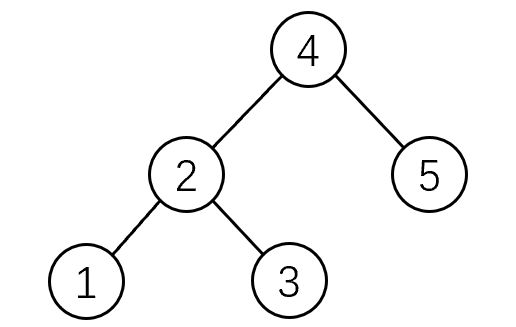
\includegraphics[width=0.22\textwidth]{assets/pics_and_ppts/ch4/20408哪一个序列不能生成图示二叉排序树.png}
\end{center}

\noindent A. 4, 5, 2, 1, 3\\
B. 4, 5, 1, 2, 3\\
C. 4, 2, 5, 3, 1\\
D. 4, 2, 1, 3, 5\\

7. 请你设计一个算法，给定任意一棵二叉树以及两个关键字a和b，返回树中a和b的最近公共祖先。假设关键字类型为int。保证树中无重复关键字并且a、b一定都存在于树中。
节点自身也被认为是自身的祖先。
\begin{cppcode}
    struct node {
        int key;
        node* lchild;
        node* rchild;
    };

    node* LowestCommonAncestor(node* root, int a, int b) {

    }
\end{cppcode}




